% ------------------------------------------------------------------------
% -*-TeX-*- -*-Hard-*- Smart Wrapping
% ------------------------------------------------------------------------
\def\baselinestretch{1}

\chapter{The Space of Lomonosov Functions}

\def\baselinestretch{1.66}

%%% ----------------------------------------------------------------------

This chapter gives a constructive proof of an abstract
approximation theorem, inspired by the celebrated result of
V.I.\,Lomonosov~\citep{Lom73}. 

\citet{AAB95} gave an alternative proof of some recent characterizations of the
invariant subspace problem. We also
establish density of non--cyclic vectors for certain convex
sets of compact quasinilpotent operators, and conclude with a
related open question. In Chapter 2 we extend the techniques
introduced in this chapter to non--compact operators acting on
a Hilbert space.

\smallskip

%%% ----------------------------------------------------------------------
\goodbreak
\section{Introduction}

\citet{Lom91} conjectured that the
adjoint of a bounded operator on a Banach space has a
non--trivial closed invariant subspace. In view of the known
examples of operators without an invariant subspace
\citep{Enf87,Rea85}, this is the strongest version of the
invariant subspace problem that can possibly have an
affirmative answer. In particular, if the Lomonosov conjecture
is true, then every operator on a reflexive Banach space has a
non--trivial invariant subspace(as shown in Figure \ref{fig1}).

\begin{figure}
\centering
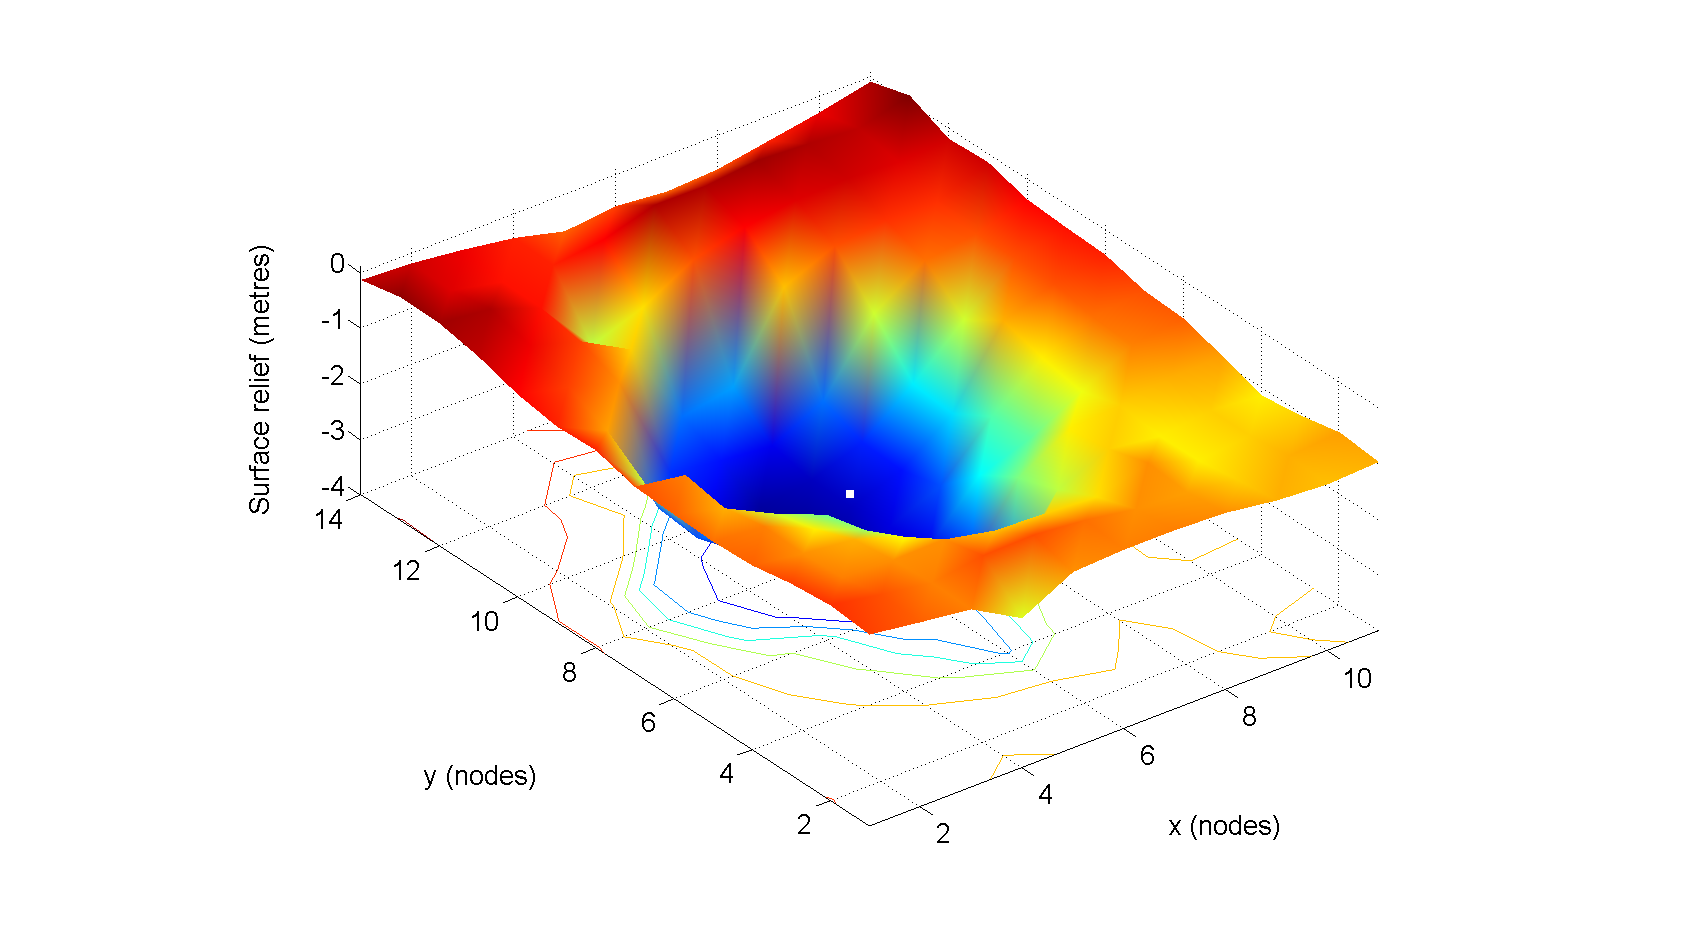
\includegraphics[scale=0.25]{fig1}
\caption{A figure sample that is not associated with the text.}
\label{fig1}
\end{figure}

\bigskip
\goodbreak

Considering the strong influence of Lomonosov's results on the
theory of invariant subspaces, it is not surprising that both
the conjecture and the techniques developed in the interesting
paper \citep{Lom91} received further attention. L.~de~Branges
used this result to obtain a characterization of the invariant
subspace problem in terms of density of certain functions. This
stimulated another characterization of the invariant subspace
problem given by Y.A.~Abramovich, C.D.~Aliprantis, and
O.~Burkinshaw ~in~\citep{AAB95}. Section~1.4 presents a more
detailed account of this work.

We take a slightly different approach. First we give a
constructive proof of the approximation theorem, inspired by
the well known Lomonosov construction used in
\citep{Lom73,RR73}. This theorem is then applied to give an
alternative proof of the main result in \citep{AAB95}. Our proof
applies to both real and complex Banach spaces, while the
original result was established for complex Banach spaces only.
The alternative proof somehow explains the role of compact
operators that appear in the characterizations of the invariant
subspace problem~\citep{AAB95}.

\medskip

\begin{table}
\caption{A sample Table}
\begin{center}
    \begin{tabular}{ | l | l | l | p{5cm} |}
    \hline
    Day & Min Temp & Max Temp & Summary \\ \hline
    Monday & 11C & 22C & A clear day with lots of sunshine.  
    However, the strong breeze will bring down the temperatures. \\ \hline
    Tuesday & 9C & 19C & Cloudy with rain, across many northern regions. Clear spells
    across most of Scotland and Northern Ireland,
    but rain reaching the far northwest. \\ \hline
    Wednesday & 10C & 21C & Rain will still linger for the morning.
    Conditions will improve by early afternoon and continue
    throughout the evening. \\
    \hline
    \end{tabular}
\end{center}
\label{tbl1}
\end{table}

One may notice that the weak*--compactness of the unit ball in
dual Banach spaces plays an important role in
\citep{AAB95,dB59,dB93,Lom91}, as well as in the applications
given in this chapter. In other words, if the Lomonosov
conjecture is true, then the compactness of the unit ball, with
respect to the weak* topology, is likely to be an important
ingredient of its proof.

\smallskip

In the last section we put this observation to the test. A
straightforward application of the approximation theorem
obtained in Section~1.3, together with the Schauder--Tychonoff
Fixed Point Theorem, yields density of non--cyclic vectors for
the dual of a convex set of compact quasinilpotent operators.
We end with the open problem of obtaining a similar result for
the original set, rather than its dual.

\bigskip

This work is more or less self--contained and the notation and
terminology used in it is (supposed to be) standard. However,
here are a few conventions that hold throughout this chapter:


\bigskip

%%% ----------------------------------------------------------------------
\goodbreak

\def\baselinestretch{1.1}

\section{Reflexive Topological Spaces and Continuous Indicator Functions}

This section introduces some topological preliminaries that
lead to a fairly general treatment of the approximation theory
in the next section, where an important role is played by the
partition of unity and the ``continuous indicator functions''
associated with a basis for the topology on a compact domain of
certain functions. The existence of continuous indicator
functions can be characterized by a purely topological property
of the underlying space, which is defined as ``reflexivity'' of
the topological space. In this section we introduce both
concepts and establish the connection between them.

\def\baselinestretch{1.66}

\begin{defn}
Let $S=(S,\tau)$ be a topological space and denote by
$C(S,\Real)$ the space of all continuous real--valued functions
on $S$. A topological space $S$ is called {\em reflexive} if
the topology $\tau$ coincides with the weakest topology
$\tau_w$ on $S$ for which all the functions in $C(S,\Real)$ are
continuous.
\end{defn}

\begin{rem}
The reflexivity of topological spaces is not to be confused
with the corresponding concept of the reflexivity of Banach
spaces. Indeed, we conclude this section by showing that every
subset of a locally convex space is reflexive.
\end{rem}

\begin{prop}
Reflexivity is a hereditary property; \, i.e. a subspace $S$ of
a reflexive topological space $X$ is reflexive with the
relative topology.
\end{prop}

\begin{proof}
Consider the restrictions of the functions in $C(X,\Real)$ to
the subset $S$, and observe that they induce the relative
topology on $S$, whenever $X$ is reflexive.
\end{proof}

\begin{defn}
Suppose $U$ is an open subset of a topological space $S$. A
continuous function $\Gamma\colon S \To \RPlus$ is called a
{\em continuous indicator function} of $U$ in $S$ if
\[ U = \set{s\in S \,\,|\,\,\, \Gamma(s) > 0}.  \]
\end{defn}

\begin{rem}
If $X$ is a metric space then every open ball
\[ U=U(x_0,r)=\set{x\in X \,\,|\,\,\, d(x,x_0) < r}, \]
admits a continuous indicator function
$\Gamma_U\colon{X}\To\RPlus$, defined by
\[ \Gamma_U(x) = \max\set{0, \, r - d(x,x_0) }. \]
Furthermore, suppose $f \in C(S,X)$. Then the open set
$V=f^{-1}(U)\subset S$ ``inherits'' an indicator function from
$U$ by setting: $\Gamma_V(s)=\Gamma_U(f(s))$.
\end{rem}

\smallskip
\goodbreak


%%% ----------------------------------------------------------------------
\goodbreak
\section{Lomonosov Functions}

The proof of the celebrated result of V.I. Lomonosov
\citep{Lom73,RR73} was based on the ingenious idea of defining a
continuous function with compact domain in a Banach space,
assuming that certain local conditions are met. In this section
we generalize this idea in the form of an approximation
theorem. Since our construction was greatly inspired by the
proof of Lomonosov's Lemma~\citep{Lom73,RR73}, we suggest the
following definition.

\begin{defn}
Let $\A \subset C(S,X)$ be a subset of the space of continuous
functions from a topological space $S$ to a locally convex
space $X$. The convex subset $\cal{L}(\A) \subset C(S,X)$,
defined by
\[ \cal{L}(\A) = \set{ \sum_{k=1}^n \alpha_k A_k \,\,|\,\,\, A_k\in\A,
   \alpha_k\in C(S,[0,1]) \text{ and } \sum_{k=1}^n\alpha_k \equiv 1;
   \,\, n < \infty}. \]

is called the {\em Lomonosov space} associated with the set
$\A$, and a function $\Lambda \in \cal{L}(\A)$ is called a {\em
Lomonosov function}.
\end{defn}

\begin{equation}
y = a + b_1x_1 + b_2x_2
\end{equation}

\medskip

Recall that the {\em uniform topology} on $C(S,X)$ is induced
by the topology on a linear space $X$. If $\cal{B}$ is a local
basis for the topology on $X$ then the sets
\[ \widehat{U}=\set{f\in C(S,X) \,\,|\,\,\, f(S)\subset U\in\cal{B}} \]
define a local basis for the uniform topology on $C(S,X)$. If
$X$ is a locally convex space then so is $C(S,X)$. In
particular, if $X$ is a Banach space then $C(S,X)$ with the
uniform topology is a Banach space, as well.

\medskip

We are now ready to give a construction of the Lomonosov
function that uniformly approximates a continuous function
within a given neighborhood.


%%% ----------------------------------------------------------------------
\goodbreak

\def\baselinestretch{1.1}

\section{Subspace Problem}

We introduce some basic concepts and notation that is
consistent with \citep{AAB95}. However, for more details and
further references on the {\em invariant subspace problem}, the
reader is advised to consult the nicely written and
comprehensible original~\citep{AAB95}.

\def\baselinestretch{1.66}
\medskip


%%% ----------------------------------------------------------------------
